
\section{The basics}

If I wish to purchase a share of a company in one year's time how much should I pay? 

The most obvious answer is that the price should reflect my expectations of the value of the company in one year, possibly adjusted for risk and discounting. This answer is wrong. In most cases the price of such a contract is fixed by arbitrage. Expectations of future value play absolutely no role in pricing such forward contracts. Nor does the riskiness of the price. Or any other considerations except the current price, the interest rate, and any financial flows (such as dividends or coupons) attached to a security.

Except for commodities, which are a little strange. 

Here we will outline the basic logic behind futures arbitrage and sketch the pricing for equities (with and without dividends), currencies, and commodities. 

\subsection{Notation}
Let the price of a security at time $0$ be $S(0)$. The price of a contract to buy or sell $S$ at a future time $T$ is $F_T(0)$. To \textbf{buy}/\textbf{sell} the future is to be obliged to buy/sell the security at $T$. Set the interest rate for a $T$ period loan at $r$. This is a \textbf{zero} rate. For simplicity we can set the zero curve at $r$ for all maturities. 

\section{What's a repo?}
To construct the arbitrage arguments we allow \textbf{short selling}. Short selling creates the opposite cash-flow as a normal purchase. Short sales are created through a transaction called a \textbf{repurchase agreement} or \textbf{repo}. 

A repo for a security $S$ involves borrowing some amount of the security and then repaying the same amount at some future time. Say we borrow at time 0 and immediately sell the security for $S(0)$ which we invest at rate $r$. We then re-acquire the security at time $T$ for $S(T)$ and repay the loan. The cash-flow generated by this transaction is $S(0)(1+r)^T-S(T)$. The opposite transaction is to borrow $S(0)$ to buy the security and then sell it at $T$ for $S(T)$. The cash-flow from this opposite transaction is $S(T) -S(0)(1+r)^T$. Figure \ref{ccrcc} illustrates. 

This is a very useful process as it gives us the mirror image payoff. This is  a useful property for arbitrage. 

\textbf{Remark: (what is the repo rate?)} Above we have assumed that someone is willing to lend the security for $T$ periods and receive no rental rate. This is somewhat unrealistic. But not too unrealistic. Provided that the security doesn't generate any payments (like dividends) the renter is not disadvantaged by the transaction: he is in precisely the same financial situation if he rents or not. He should therefore be indifferent between renting and not renting and so only require a small compensation (a small rate $\epsilon$, or, if you like, a cheap brass trinket). Of course he would prefer more but competitive pressures force him to accept the trinket or settle for nothing.

Owners of securities are regularly paid non-trivial rental rates (\textbf{repo rates}). There are various reasons for this: there is a credit risk associated with the loan (though this can be reduced to a trivial level by margining the loan). If a stock pays dividends the lender will need to be compensated for the loss, but as we will see this and other flows like bond coupons can easily be incorporated into the futures price. There's another big reason, possibly the main reason, but we'll get to that later.

\section{Arbitrage pricing with futures}
 
Futures are priced by constructing arbitrage portfolios that hedge the exposure from the long or short future. The arbitrage process for a short future is called \textbf{cash and carry}; for a long future it is called \textbf{reverse cash and carry}. 

\begin{itemize}
\item \textbf{The cash and carry portfolio}: Buy the security with borrowed money and hold. Sell the futures contract. 
\item \textbf{The reverse cash and carry portfolio}: Repo the security, sell at market, and invest at the risk free rate. Buy the futures contract.
\end{itemize}


%model
%\begin{tiny}
%\begin{tabular}{cc|c|c}
%&$\rightarrow$ & Deliver stock for $F_T(0)$ & T\\ 
% & & Repay loan: $S(0)(+r)^T$ & \\
%\hline
%\textsc{Cash and carry}&$\uparrow$ & & Receive stock for $F_T(0)$\\
%& Sell future @ $F_{T}(0)$    & &   Receive proceeds of loan: $S(0)(1+r)^T$ \\
%& Borrow cash $S(0)$ @ $r$ & & Repay repo \\
%& Buy stock @ $S(0)$ (hold)  & & \\
%\hline
%& 0  & Buy future @ $F_{T}(0)$ $\rightarrow$ & $\uparrow$ \\
%& &  Borrow stock & \\
%&& Sell stock @ $S(0)$ & \\
%&  & Invest $S(0)$ @ $r$ & \\
%& & \textsc{Reverse cash and carry} & \\
%\end{tabular}
%\end{tiny}


\begin{tiny}
\begin{table}
\begin{tabular}{cc|c|c}
&$\rightarrow$ & Deliver stock & T\\ 
 & & Repay loan & \\
\hline
\textsc{Cash and carry}&$\uparrow$ & & Receive stock\\
& Sell future    & &   Receive proceeds of loan \\
& Borrow cash & & Repay repo \\
& Buy stock (hold)  & & \\
\hline
& 0  & Buy future  $\rightarrow$ & $\uparrow$ \\
& &  Borrow stock & \\
&& Sell stock  & \\
&  & Invest cash & \\
& & \textsc{Reverse cash and carry} & \\
\end{tabular}\label{ccrcc}
\caption{Cash and carry and reverse cash and carry}
\end{table}
\end{tiny}


We'll consider four cases: equities with and without dividends, currencies, and commodities. These are arranged from least to most complicated. We'll use discrete compounding to make the analysis simple. The continuously compounded results are straightforward extensions.

\subsection{Equity futures}


\subsubsection{General case}

\textit{Cash and carry:}

\begin{center} \begin{tabular}{|c|c|}
  \hline
  % after \\: \hline or \cline{col1-col2} \cline{col3-col4} ...
  time & action \\
  \hline
  t & Sell future @ $F_{T}(0)$  \\
    & Borrow cash $S(0)$ @ $r$ \\
    & Buy stock @ $S(0)$ (hold) \\
  \hline
 T & Deliver stock for $F_T(0)$ \\
   & Repay loan: $S(0)(+r)^T$ \\
  \hline
   & $F_{T}(0) - S(0)(1+r)^{T}$\\
  \hline
\end{tabular}\end{center}

\textit{Reverse cash and carry:}

\begin{center} \begin{tabular}{|c|c|}
  \hline
  % after \\: \hline or \cline{col1-col2} \cline{col3-col4} ...
  time & action \\
  \hline
  t & Buy future @ $F_{T}(0)$  \\
    & Borrow stock \\
    & Sell stock @ $S(0)$  \\
    & Invest $S(0)$ @ $r$\\
  \hline
  T & Receive stock for $F_T(0)$ \\
    & Receive proceeds of loan: $S(0)(1+r)^T$\\
    & Repay repo \\
  \hline
   & $S(0)(1+r)^{T}-F_{T}(0)$\\
  \hline
\end{tabular}\end{center}

Both these transactions cannot be profitable for there to be no arbitrage. This requires

\[S(0)(1+r)^{T}-F_{T}(0) \leq 0 \]
and
\[F_{T}(0)-S(0)(1+r)^{T} \leq 0 \]
which implies
\[ F_{T}(0) = S(0)(1+r)^{T}  \]

\subsubsection{Example}

\textbf{Non dividend paying stock}

Current price: $S(0)$ = \$100\\
Borrowing/lending: $r$ = 0.05\\
Futures expiry: 1 year\\
Futures price: 100(1+0.05) = \$105 

\subsubsection{Arbitrage}


Say future is 110:

\begin{center} \begin{tabular}{|c|c|}
  \hline
  % after \\: \hline or \cline{col1-col2} \cline{col3-col4} ...
  time & action \\
  \hline
  t & Sell future @ 110  \\
    & Borrow cash \$100 @ 0.05 \\
    & Buy stock @ $100$ (hold) \\
  \hline
 T & Deliver stock for 100 \\
   & Repay loan: $100(1+0.05)^1$ \\
  \hline
   & $110 - 100(1+0.05)^1 = 5 >0$ (free profit)\\
  \hline
\end{tabular}\end{center}

Say future is 100:

\begin{center} \begin{tabular}{|c|c|}
  \hline
  % after \\: \hline or \cline{col1-col2} \cline{col3-col4} ...
  time & action \\
  \hline
  t & Buy future @ 100  \\
    & Borrow stock \\
    & Sell stock @ 100  \\
    & Invest \$100 @ 0.05\\
  \hline
  T & Receive stock for 100 \\
    & Receive proceeds of loan: $100(1+0.05)^1$\\
    & Repay repo \\
  \hline
   & $100(1+0.05)^1-100 = 5 >0$\\
  \hline
\end{tabular}\end{center}

For no arbitrage to hold we must have $F_{T}(0) = 100(1+0.05)^{1} = 105$

\subsection{Equity futures with dividends}

The holder of a stock receives the dividend so the stock lender has to be compensated for their lost dividend. We will assume that the dividend is paid as a proportion of the futures price. This seems a little strange but it makes the calculation easier.

\subsubsection{General case}

\textit{Cash and carry:}

\begin{tiny}
\begin{center} \begin{tabular}{|c|c|}
  \hline
  % after \\: \hline or \cline{col1-col2} \cline{col3-col4} ...
  time & action \\
  \hline
  t & Sell future @ $F_T(0)$  \\
    & Borrow cash $S(0)$ @ $r$ \\
    & Buy stock @ $S(0)$ (hold) \\
  \hline
 T & Deliver stock for $F_T(0)$ \\
   & Repay loan $S(0)(1+r)^{T}$\\
   & Receive dividend $F_T(0)((1+d)^{T}-1)$\\
  \hline
   & $F_T(0) - S(0)(1+r)^{T} + F_T(0)((1+d)^{T}-1)$\\
  \hline
\end{tabular}\end{center}
\end{tiny}

\textit{Reverse cash and carry:}

\begin{tiny}
\begin{center} \begin{tabular}{|c|c|}
  \hline
  % after \\: \hline or \cline{col1-col2} \cline{col3-col4} ...
  time & action \\
  \hline
  t & Buy future @ $F_T(0)$  \\
    & Borrow stock \\
    & Sell stock @ $S(0)$  \\
    & Invest $S(0)$ @ $r$\\
  \hline
  T & Receive stock for $F_T(0)$ \\
    & Receive proceeds of loan: $S(0)(1+r)^{T}$\\
    & Repay repo \\
    & Pay dividend $F_T(0)((1+d)^{T}-1)$\\
  \hline
   & $S(0)(1+r)^{T}-F_T(0) - F_T(0)((1+d)^{T}-1)$\\
  \hline
\end{tabular}\end{center}
\end{tiny}

Both these transactions cannot be profitable for there to be no arbitrage. this requires

\[S(0)(1+r)^{T}-F_T(0) - F_T(0)((1+d)^{T}-1) \leq 0 \]
\[F_T(0) - S(0)(1+r)^{T} + F_T(0)((1+d)^{T}-1) \leq 0 \]
\[ \Rightarrow F_T(0) = S(0)\frac{(1+r)^{T}}{(1+d)^{T}}  \]

\subsubsection{Example}
Current price: $S(0)$ = \$100\\
Borrowing/lending: $r$ = 0.05\\
Dividend rate: $d$ = 0.02\\
Futures expiry: 1 year\\
Futures price: 100(1+0.05)/(1+0.02) = \$101.9417 

\subsubsection{Arbitrage}


Say future is 110:

\begin{tiny}
\begin{center} \begin{tabular}{|c|c|}
  \hline
  % after \\: \hline or \cline{col1-col2} \cline{col3-col4} ...
  time & action \\
  \hline
  t & Sell future @ 110  \\
    & Borrow cash \$100 @ 0.05 \\
    & Buy stock @ $100$ (hold) \\
  \hline
 T & Deliver stock for 110 \\
   & Repay loan: $100(1+0.05)^1$ \\
   & Receive dividend payment  $100((1+0.02)^1-1)$\\
  \hline
   & $110 - 100(1+0.05)^1+ 100((1+0.02)^1-1)  >0$ (free profit)\\
  \hline
\end{tabular}\end{center}
\end{tiny}

Say future is 100:

\begin{tiny}
\begin{center} \begin{tabular}{|c|c|}
  \hline
  % after \\: \hline or \cline{col1-col2} \cline{col3-col4} ...
  time & action \\
  \hline
  t & Buy future @ 100  \\
    & Borrow stock \\
    & Sell stock @ 100  \\
    & Invest \$100 @ 0.05\\
  \hline
  T & Receive stock for 100 \\
    & Receive proceeds of loan: $(1+0.05)^1$\\
    & Pay dividend: $100((1+0.02)^1-1)$ \\
    & Repay repo\\
  \hline
   & $100(1+0.05)^1-100((1+0.02)^1-1)-100 >0$\\
  \hline
\end{tabular}\end{center}
\end{tiny}

For no arbitrage to hold we must have $F_{T}(0) = 100\frac{(1+0.05)^{1}}{(1+0.03)^1} = 101.9417$

\subsection{Currency}

Currencies are a slightly more interesting case. The arbitrage portfolios involve borrowing and lending in two currencies with different interest rates. The price of a futures contract incorporates the difference between interest rates; if the rates are the same the futures price is the same as the spot price.

Since the arbitrage portfolios involve borrowing and lending futures contracts have the same characteristics as a foreign denominated loan financed with domestic currency or visa-versa. This is a useful characteristic: it means if you can borrow in one currency you can borrow in all currencies where futures contracts are traded. An Australian businessman might tire of paying high interest rates in his home country and buy a futures contract that swaps his exposure into Japanese yen or Swiss francs to take advantage of the lower interest rate. 

Imagine a \textbf{domestic} currency with interest rate $r_d$ and a \textbf{foreign} currency with interest rate $r_f$. As before we assume that an unlimited amount of money can be borrowed or lent at these rates at all maturities.  

\subsubsection{General case}


Exchange rate (domestic for foreign): $S(t)$\\
Domestic interest rate: $r_d$\\
Foreign interest rate: $r_f$\\
Future exchange rare (domestic for foreign): $F_T(t)$\\
Initial domestic borrowing $B$

\textit{Cash and carry:}

\begin{center} \begin{tabular}{|c|c|}
  \hline
  % after \\: \hline or \cline{col1-col2} \cline{col3-col4} ...
  time & action \\
  \hline
  %t & Sell $\frac{B}{S(t)}$ futures @ $F_{T}(t)$  \\
   t & Borrow domestic cash $B$ @ $r_d$ \\
    & Lend foreign cash $\frac{B}{S(t)}$ @ $r_f$  \\
  \hline
 T & Repay domestic loan $B(1+r_d)^{T}$ \\
   & Receive foreign loan $\frac{B}{S(t)}(1+r_f)^{T}F_T(t)$   \\
   & (converted into domestic currency)\\
  \hline
   & $\frac{B}{S(t)}(1+r_f)^{T}F_T(t)-B(1+r_d)^{T}$\\
  \hline
\end{tabular}\end{center}

\textit{Reverse cash and carry:}

\begin{center} \begin{tabular}{|c|c|}
  \hline
  % after \\: \hline or \cline{col1-col2} \cline{col3-col4} ...
  time & action \\
  \hline
  %t & Buy $\frac{B}{S(t)}$ futures @ $F_{T}(t)$  \\
  T  & Borrow foreign cash $\frac{B}{S(t)}$ @ $r_f$ \\
    & Lend domestic cash $B$ @ $r_d$  \\
  \hline
  T & Repay foreign loan $\frac{B}{S(t)}(1+r_f)^{T}F_T(t)$  \\
    & (converted into domestic currency) \\
   & Receive domestic loan $B(1+r_d)^{T}$ \\
  \hline
   & $B(1+r_d)^{T}-\frac{B}{S(t)}(1+r_f)^{T}F_T(t)$\\
  \hline
\end{tabular}\end{center}


Both these transactions cannot be profitable for there to be no arbitrage. this requires

\[\frac{B}{S(t)}(1+r_f)F_T(t)-B(1+r_d)^{T} \leq 0 \]
\[B(1+r_d)^{T}-\frac{B}{S(t)}(1+r_f)^{T}F_T(t) \leq 0 \]
\[ \Rightarrow F_{T}(t) = S(t)\frac{(1+r_d)^{T}}{(1+r_f)^{T}}  \]



\subsubsection{Example}


Exchange rate (domestic for foreign): 2\\
Domestic interest rate: 0.05\\
Foreign interest rate: 0.1\\
Future exchange rare (domestic for foreign): 1.95\\

\subsubsection{Arbitrage}

Domestic currency is suffixed with a 'd' and foreign currency with an 'f'. Initial domestic borrowing 100d. As in the equities example we'll price the future incorrectly and show the arbitrage both sides.

\textit{Cash and carry:}

If $F_T(t)=1.95$

\begin{center} \begin{tabular}{|c|c|}
  \hline
  % after \\: \hline or \cline{col1-col2} \cline{col3-col4} ...
  time & action \\
  \hline
  %t & Sell $\frac{B}{S(t)}$ futures @ $F_{T}(t)$  \\
   t & Borrow domestic cash 100d @ 0.05 \\
    & Lend foreign cash $\frac{100}{2} = 50f$ @ $0.1$  \\
  \hline
 T & Repay domestic loan $100(1+0.05)^{1} = 105d$ \\
   & Receive foreign loan $\frac{100}{2}(1+0.1)^{1}1.95 = 50*1.1*1.95 = 107.25d$ \\
   &  (converted into domestic currency) \\
  \hline
   & $107.25d-105d = 2.25d$\\
  \hline
\end{tabular}\end{center}

\textit{Reverse cash and carry:}

If $F_T(t)=1.85$

\begin{center} \begin{tabular}{|c|c|}
  \hline
  % after \\: \hline or \cline{col1-col2} \cline{col3-col4} ...
  time & action \\
  \hline
  %t & Buy $\frac{B}{S(t)}$ futures @ $F_{T}(t)$  \\
  T  & Borrow foreign cash $\frac{100}{2} = 50f$ @ $0.1$ \\
    & Lend domestic cash $100d$ @ $0.05$  \\
  \hline
  T & Repay foreign loan $\frac{100}{2}(1+0.1)^{1}1.85 = 50*1.1*1.85 = 101.75d$ \\
  & (converted into domestic currency)  \\
   & Receive domestic loan $100(1+0.05)^{1} = 105d$ \\
  \hline
   & $105-101.75 = 3.25d$\\
  \hline
\end{tabular}\end{center}


The correct forward price is the price at which neither of these sequences of trades are profitable:
\[ F_{T}(t) = 2\frac{(1+0.05)^1}{(1+0.1)^1} = 1.9091 \]

%\subsubsection{Swapping a loan with a currency futures contract}

%Say that 


\subsection{Commodities}


Commodity futures are a little odd because it is often difficult to borrow the commodity to effect a short sale. This means that the reverse cash and carry is impossible and there is only an upper bound provided by the cash and carry arbitrage. As a consequence the futures price can incorporate price and risk expectations to an extent. 

The futures price also incorporates the value of holding the physical commodity before maturity. This value is called the \textbf{convenience yield}. To understand the convenience yield consider a person who holds the physical commodity at time $0$. How much would such a person need to be compensated to give up the right to sell the commodity between $0$ and $T$? The appropriate value of compensation is the convenience yield for a futures contract delivered at $T$.  

Risk will be priced in the futures, but can have a positive or negative effect on price. An oil producer might fear a price crash and so offer a discount on the futures contract; however oil buyers might fear a price spike and so pay more. The net effect depends whether buyers or sellers are more risk averse.

Due to the absence of a lower bound futures prices have a \textbf{term structure} very much like interest rates. If futures prices are higher than spot the commodity is in \textbf{contango}, if it is lower the commodity is in \textbf{backwardation}. 

\begin{figure}[htbp]
\begin{center}
  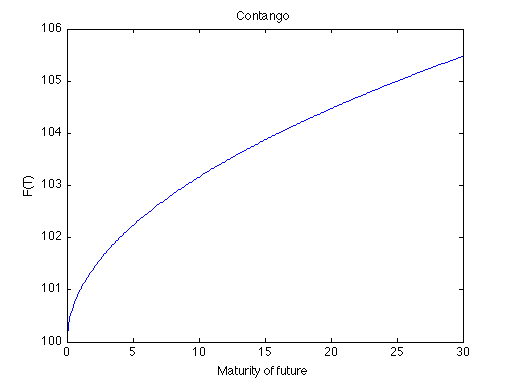
\includegraphics[width=2in]{pics/contango.png} 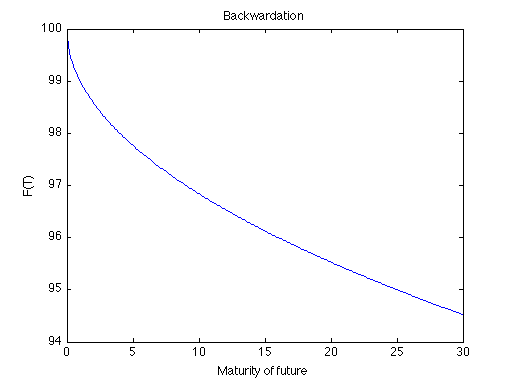
\includegraphics[width=2in]{pics/backwardation.png}   \caption{Contango and backwardation}
\label{contangoandbackwardation}
\end{center}
\end{figure}
\subsubsection{General case}

In order to hold a physical commodity for the cash and carry it is necessary to pay for storage (and possibly for any spoilage in the commodity). The storage cost can be treated much like a negative dividend. We will call the storage rate $s$.

\textit{Cash and carry:}


\begin{center} \begin{tabular}{|c|c|}
  \hline
  % after \\: \hline or \cline{col1-col2} \cline{col3-col4} ...
  time & action \\
  \hline
  t & Sell future @ $F_T(0)$  \\
    & Borrow cash $S(0)$ @ $r$ \\
    & Buy commodity @ $S(0)$ (hold in storage) \\
  \hline
 T & Deliver commodity for $F_T(0)$ \\
   & Repay loan: $S(0)(1+r)^{T} $ \\
   & Pay storage cost $F_T(0)((1-s)^{T}-1)$\\
  \hline
   & $F_T(0) - S(0)(1+r)^{T} + F_T(0)((1-s)^{T}-1)$\\
  \hline
\end{tabular}\end{center}


This transactions cannot be profitable under no arbitrage. This requires

\[F_T(0) - S(0)(1+r)^{T} + F_T(0)((1-s)^{T}-1) \leq 0 \]
\[ \Rightarrow F_T(0) = S(0)\frac{(1+r)^{T}}{(1-s)^{T}}  \]

\subsubsection{Example}

Current price: $S(t)$ = \$61\\
Borrowing/lending: $r$ = 0.05\\
Storage cost: $s$ = 0.07\\
Futures expiry: 30 days\\
Futures price upper  bound: $61((1+0.05)/(1-0.02))^{30/365}$ = \$61.35

\subsubsection{Arbitrage}

Spot crude oil sells for \$61 on June 30. A contract for delivery on July 30 delivery sells for \$64. It costs 7\% per year to store and transport the oil. The interest rate is 5\%.

\textit{Cash and carry:}

\begin{center} \begin{tabular}{|c|c|}
  \hline
  % after \\: \hline or \cline{col1-col2} \cline{col3-col4} ...
  time & action \\
  \hline
  June 30 & Sell future @ $64$  \\
    & Borrow cash $61$ @ $0.05$ \\
    & Buy commodity @ $61$ (hold in storage) \\
  \hline
 T & Deliver commodity for $64$ \\
   & Repay loan: $61(1+0.05)^1$ \\
   & Pay storage cost $64((1-0.07)^{30/365}-1)$\\
  \hline
   & $64 - 61(1+0.05)^{30/365} + 64((1-0.07)^{30/365}-1) = 2.3743$\\
  \hline
\end{tabular}\end{center}

So if the future trades at \$64 (or above) the cash and carry transaction is profitable.

\section{The operation of real world futures contracts}

Real world futures contracts have a few more complications than the examples above. The financial exposure of a contract is typically a multiple of the actual futures price. For example a NYMEX contract for oil is quoted in dollars per barrel, but the contract is actually for 1000 barrels, so if the futures price is \$70, the total value of the oil traded is \$70,000. Equity index and currency contracts are similarly multiples of the quoted price.

Exchange traded futures contracts typically use a process called \textbf{margining} to reduce credit risk. The long and short contractees each have \textbf{margin accounts} containing a fraction of the total value of the contracts (typically around 10\%). Margin accounts are are used to finance short term moves in the value of the contracts. If a margin account balance gets too low a \textbf{margin call} occurs: the account must be topped up or the position closed with an offsetting trade. Because margining occurs daily, and the margin accounts are large enough to finance a large move in the underlying price, there is greatly reduced risk that someone who enters into a futures contract will default on their obligations. 

Margining also allows for substantial \textbf{leverage} since only a fraction of the total exposure is required in the margin account to sustain a position. 

Consider an example: Say we hold 50 futures contracts on a security priced in domestic currency. The contract size is \$1000 $\times$ the underlying security price. Let's see what happens when the contract price moves from 100 to 105 if the margin is 10\% of total contract value.

\begin{center} \begin{tabular}{|c|c|c|}
  \hline
  % after \\: \hline or \cline{col1-col2} \cline{col3-col4} ...
  Today& price & 100 \\
  & contract value & \$100,000 \\
  & value of portfolio & \$5,000,000 \\
  & margin & \$500,000 \\
   \hline
  Tomorrow & price & 105 \\
  & contract value & \$105,000 \\
  & value of portfolio & \$5,250,000 \\
  & margin & \$525,000 \\
  \hline
\end{tabular}\end{center}

The position has a profit of \$5,250,000-\$5,000,000 = \$250,000. The margin increases by \$25,000. The long position receives \$225,000 (250,000-25,000) in additional cash and has a profit of \$250,000. A \$250,000 return on an initial margin of \$500,000 for a 5\% move represents a lot of leverage. However typically a portfolio funding a futures position will have substantially more than the margin. If the concept of leverage is sensible (and it often isn't) it's more natural to measure the return against the portfolio capital. In the previous example the portfolio might be \$10,000,000 (return would be 2.5\%) or \$1,000,000 (return would be 25\%).

\section{Margining and why currency risk doesn't matter much}

Futures contracts are denominated in currency, usually US dollars. It seems logical that the futures carry a full exposure to currency moves: logical but wrong. Provided that the profit or loss is margined regularly the currency exposure is very limited. We can see this by considering the effect of a currency move on the cashflows from a futures contract. To make things simple we'll consider a futures contract on a non-dividend paying equity. In the example we have an US dollar denominated futures contract and an Australian dollar denominated bank account.

Say initially the currencies are at parity (USD1 = AUD1) and the futures price is USD100. Overnight the Australian dollar devalues to USD0.9. The value of a portfolio containing one futures contract is affected as follows.


\begin{center} \begin{tabular}{|c|c|c|}
  \hline
  % after \\: \hline or \cline{col1-col2} \cline{col3-col4} ...
  Today& price & USD100 \\
  & contract value & USD100,000 \\
  & value of portfolio & USD100,000 (AUD100,000) \\
  & margin & USD10,000 (AUD10,000) \\
   \hline
  Tomorrow & price & USD100 \\
  & contract value & USD100,000 (AUD90,000) \\
  & value of portfolio &USD100,000(AUD90,000)  \\
  & margin & USD10,000 (AUD9,000) \\
  \hline
\end{tabular}\end{center}

Our margin account denominated in USD has decreased in value by AUD1000 which is quite small considering the size of the currency move. This is because currency changes only affect the margin which is typically only a portion of the total portfolio value.


\section{Questions}

\textbf{Question 1:}\\

Consider a non-dividend paying stock in the following situation:

\begin{center}
\begin{tabular}{|c|}
\hline
Current price: $S(t)$ = \$14.5\\
Borrowing/lending: $r$ = 0.1\\
Futures expiry: 1 year\\
Futures price: \$14.5\\
\hline
\end{tabular}
\end{center}

\textbf{(a)} Construct an arbitrage to take advantage of the mispricing. How much money can you make?\\
\textbf{(b)} Redo part (a) assuming the repo rate is 2\% per year.

\medskip

\textbf{Question 2:}\\

Consider the following situation in the foreign exchange market:

\begin{center}
\begin{tabular}{|c|}
\hline
Exchange rate (domestic for foreign): 0.67\\
Domestic interest rate: 0.15\\
Foreign interest rate: 0.01\\
Future exchange rate (domestic for foreign): 0.68\\
\hline
\end{tabular}
\end{center}

\textbf{(a)} Construct an arbitrage to take advantage of the mispricing. 

\medskip

\textbf{Question 3:}\\

Consider the following situation in the market for gold:

Spot gold sells for \$900 on June 30. A contract for delivery on August 30 delivery sells for \$920. It costs 1\% per year to store. The interest rate is 5\%.

\textbf{(a)} Construct an arbitrage to take advantage of the mispricing. \\
\textbf{(b)} Suppose instead that the forward price was \$900.1 and it is possible to repo gold for 0.5\% per year. Construct the arbitrage.

\medskip

\textbf{Question 4:}\\


\textbf{(a)} Consider the futures contract in the picture. If you currently hold 100 of these contracts on 10\% margin and the futures price moves to \$70 overnight what are your cashflows in USD?\\
\textbf{(b)} What are your cashflows in AUD assuming that the exchange rate is constant at 0.7.\\
\textbf{(c)} What are your cashflows in AUD assuming that the exchange rate moves from 0.7 to 0.62.

\begin{center}
  % Requires \usepackage{graphicx}
  \includegraphics[width=5in]{pics/cln9des} \\
  \textit{Futures contract on crude oil}
\end{center}

